\documentclass[11pt,a4paper]{article}
\usepackage[T1]{fontenc}
\usepackage[utf8]{inputenc}
\usepackage{lmodern}
\usepackage{amsmath,amssymb,amsthm,mathtools,mathrsfs}
\usepackage{graphicx,float,xcolor,multicol}
\usepackage[shortlabels]{enumitem}
\usepackage[margin=27mm]{geometry}
\usepackage{microtype,needspace,placeins}
\usepackage{tikz,tikz-cd}
\usetikzlibrary{arrows.meta,calc,positioning,patterns,decorations.pathreplacing}
\usepackage[colorlinks=true,linkcolor=teal,urlcolor=teal,citecolor=teal]{hyperref}
\setlength{\parindent}{0pt}
\setlength{\parskip}{.6em}
\setcounter{secnumdepth}{0}
\allowdisplaybreaks
\raggedbottom
\providecommand{\cross}{\times}
\DeclareUnicodeCharacter{2020}{\ensuremath{\dagger}}
\DeclareMathOperator{\supp}{supp}
\DeclareMathOperator*{\esssup}{ess\,sup}
\providecommand{\chapter}{\section}
\newenvironment{tool}[2]{\subsection*{Tool #1 --- #2}}{}
\newcommand{\ToolRef}[1]{Tool #1}
\newcommand{\FigureTag}[2]{\textit{Figure #1}}
\newcommand{\Result}[1]{\subsection*{#1}}
\newcommand{\Application}[1]{\subsubsection*{Application\if\relax\detokenize{#1}\relax\else\space--- #1\fi}}
\newcommand{\ProofHeading}{\par\textit{Proof.}\space}
\newcommand{\ProofOf}[1]{\par\textit{Proof of #1.}\space}
\newcommand{\RemarkHeading}{\par\textbf{Remark.}\space}
\newcommand{\NoteHeading}{\par\textbf{Note.}\space}
\newcommand{\ExerciseHeading}{\par\textbf{Exercise.}\space}

% Rendering support only; mathematical text is in each independent post.
\usepackage{booktabs,array,longtable}
\definecolor{HandoutBlue}{HTML}{2F6690}
\definecolor{HandoutNavy}{HTML}{17365D}
\newtheorem{theorem}{Theorem}
\newtheorem{lemma}[theorem]{Lemma}
\newtheorem{proposition}[theorem]{Proposition}
\newtheorem{corollary}[theorem]{Corollary}
\newtheorem{conjecture}[theorem]{Conjecture}
\newtheorem{definition}{Definition}
\newtheorem{example}{Example}
\newtheorem{namedtoolcounter}{Tool}
\newenvironment{namedtool}[1]{\begin{namedtoolcounter}[#1]}{\end{namedtoolcounter}}
\newtheorem*{claim}{Claim}
\newtheorem*{remark}{Remark}
\newtheorem*{exercise}{Exercise}
\newtheorem*{question}{Question}
\newtheorem*{observation}{Observation}
\newcommand{\SourceChapter}[2]{\section*{#2}}
\newcommand{\Lecture}[2]{\section*{Lecture #1: #2}}
\newcommand{\unclear}[1]{\textit{[unclear: #1]}}
\newcommand{\sourcegap}{\textit{[unfinished in the source]}}
\DeclareMathOperator{\dist}{dist}
\DeclareMathOperator{\id}{id}
\DeclareMathOperator{\Hol}{Hol}
\DeclareMathOperator{\Per}{Per}
\DeclareMathOperator{\Fix}{Fix}
\DeclareMathOperator{\diam}{diam}
\DeclareMathOperator{\Var}{Var}
\DeclareMathOperator{\Leb}{Leb}
\DeclareMathOperator{\Hom}{Hom}
\DeclareMathOperator{\End}{End}
\DeclareMathOperator{\Ann}{Ann}
\DeclareMathOperator{\Spec}{Spec}
\DeclareMathOperator{\Max}{Max}
\DeclareMathOperator{\Ob}{Ob}
\DeclareMathOperator{\Tor}{Tor}
\DeclareMathOperator{\Ass}{Ass}
\DeclareMathOperator{\Mor}{Mor}
\DeclareMathOperator{\Fun}{Fun}
\DeclareMathOperator{\Nat}{Nat}
\DeclareMathOperator{\Cone}{Cone}
\DeclareMathOperator{\MCG}{MCG}
\DeclareMathOperator{\Aut}{Aut}
\DeclareMathOperator{\Deck}{Deck}
\DeclareMathOperator{\SL}{SL}
\DeclareMathOperator{\PSL}{PSL}
\DeclareMathOperator{\Area}{Area}
\DeclareMathOperator{\im}{im}
\DeclareMathOperator{\PSh}{PSh}
\newcommand{\CRing}{\mathsf{CRings}}
\newcommand{\AMod}{A\text{-}\mathsf{Mod}}
\newcommand{\Ab}{\mathsf{Ab}}
\newcommand{\Z}{\mathbb Z}
\newcommand{\Q}{\mathbb Q}
\newcommand{\R}{\mathbb R}
\newcommand{\C}{\mathbb C}
\newcommand{\N}{\mathbb N}
\newcommand{\kk}{\mathbb k}
\renewcommand{\aa}{\mathfrak a}
\newcommand{\bb}{\mathfrak b}
\newcommand{\pp}{\mathfrak p}
\newcommand{\qq}{\mathfrak q}
\newcommand{\mm}{\mathfrak m}
\newcommand{\nn}{\mathfrak n}
\newcommand{\rad}{\mathrm r}
\newcommand{\cat}[1]{\mathsf{#1}}
\setcounter{secnumdepth}{0}
\allowdisplaybreaks

\graphicspath{{figures/lemma-book/}}
\begin{document}
\section*{Working Backwards, Area Ratios, and Geometric Constructions}
% BLOG-CONTENT-BEGIN
% Source page 12 - left
\setcounter{theorem}{33}\begin{lemma}[A working-backwards strategy]\label{lemma:lb1-39}
Another major lemma is the strategy of working backwards, in a slightly different version used here to resolve problems.
First read the statement. If it asks to prove that ``$A$ holds if and only if $B$ is true,'' then, for this type of problem, begin by showing that if $A$ holds, $B$ follows. This discovers one direction; both implications must ultimately be proved.
\end{lemma}

Consider the following geometry problem from IMO 1994, problem 2.
Let $ABC$ be an isosceles triangle with $AB=AC$.
Let $M$ be the midpoint of $BC$, and let $O$ lie on line $AM$ with $OB\perp AB$.
Let $Q$ be on segment $BC$, distinct from $B,C$.
Let $E$ lie on line $AB$ and $F$ on line $AC$, with $E,Q,F$ distinct and collinear.
Prove that $OQ\perp EF$ if and only if $QE=QF$.

\paragraph{Trailer.}
Let $E$ and $F$ lie on the same side of $Q$, as shown.
\begin{figure}[H]\centering
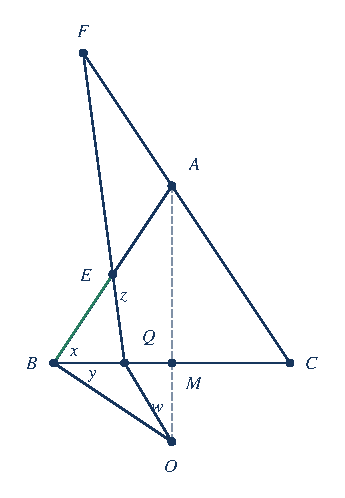
\includegraphics[width=.56\linewidth]{lb1-fig-05.pdf}
\FigureTag{LB1.5}{fig:lb1-05}
\end{figure}
Write $\angle EQM=x+z$ and $\angle OQM=y+w$.
Then $\angle EQO=(x+y)+(z+w)=\pi/2+k$.
For $OQ\perp EQ$, $k=0$, so $z=w=0$.
But this requires $Q=B$ or $Q=C$, contrary to the assumption.
Thus $E,F$ cannot both lie on the same side of $Q$.

\paragraph{Movie.}
We first show that $OQ\perp EF$ implies $QE=QF$.
\begin{figure}[H]\centering
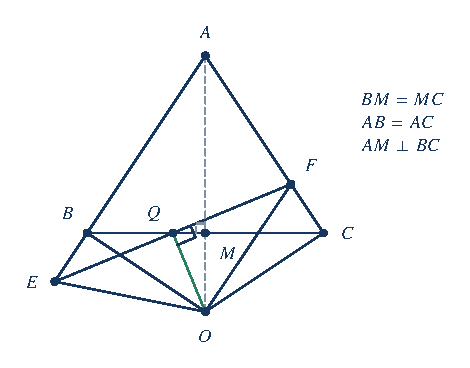
\includegraphics[width=.62\linewidth]{lb1-fig-06.pdf}
\FigureTag{LB1.6}{fig:lb1-06}
\end{figure}
$OQBE$ is cyclic, so $\angle QOE=\angle QBA=x$, say.
Then $\angle MBA=\angle BOM=x$. By symmetry of the figure, $\angle BOM=\angle MOC=x$.
Also $\angle MBA=\angle MCA=x$, so $\angle MCO=\pi/2-\angle MOC=\pi/2-x$.
Thus $\angle ACO=(\pi/2-x)+x=90^\circ$.
Consequently $QOCF$ is cyclic, and $\angle QCF=\angle QOF=x=\angle QOE$.
This establishes $QE=QF$.

Conversely, put $A=(0,a)$, $B=(-b,0)$ and $C=(b,0)$. Then
$M=(0,0)$, and $OB\perp AB$ gives $O=(0,-b^2/a)$.
Write $Q=(q,0)$. If $QE=QF$, then $Q$ is the midpoint of $EF$.
Since $E\in AB$ and $F\in AC$, this gives
\[
 E=(q-b,aq/b),\qquad F=(q+b,-aq/b).
\]
Hence
\[
 \overrightarrow{EF}=(2b,-2aq/b),\qquad
 \overrightarrow{OQ}=(q,b^2/a),
\]
and $\overrightarrow{EF}\cdot\overrightarrow{OQ}=0$.
Therefore $OQ\perp EF$.

\setcounter{theorem}{34}\begin{lemma}[Caution with the strategy]
Lemma~\ref{lemma:lb1-39} cannot be applied very easily. Since it is a new technique, it can lead to a major error if the final argument is not formed correctly.
Here we exploited the fact that a statement $B$ in mathematical logic has only two truth values, true or false.
There are statements with more than two truth values; anyway, for Olympiad business it is well and good. Discovering a necessary intermediate statement does not by itself prove the original claim.
\end{lemma}

% Source page 13 - left
Many combinatorial geometry problems are based on very elementary geometry.
It is therefore worth glancing at some lesser-known theorems.
\setcounter{theorem}{35}\begin{lemma}[Pascal's theorem]
If $A,X,A'$ and $B,Y,B'$ are collinear in the two-circle configuration, then $AB\parallel A'B'$.
\end{lemma}
\begin{figure}[H]\centering
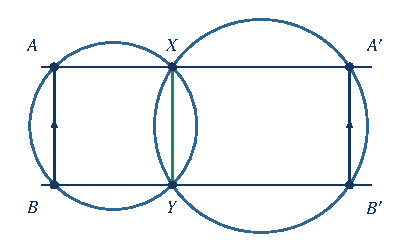
\includegraphics[width=.76\linewidth]{lb1-fig-07.pdf}
\FigureTag{LB1.7}{fig:lb1-07}
\end{figure}
This simple theorem is often neglected by Olympiad students; as a result, they have difficulty solving the following problem.

Two circles intersect at $X,Y$. Draw a chord $AB$ in the first circle.
Extend $AX,BY$ to meet the second circle at $A',B'$.
Construct a circle through $A',B'$, and extend $XA',YB'$ to meet the third circle at $A^2,B^2$.
Iterate this $2014$ times. Determine the number of trapeziums in the resulting configuration.
\begin{figure}[H]\centering
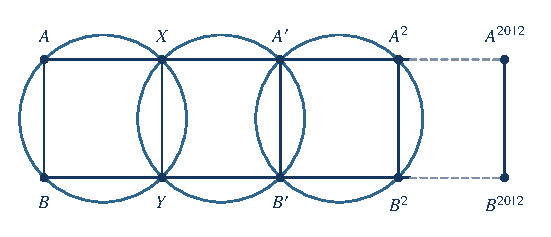
\includegraphics[width=.90\linewidth]{lb1-fig-08.pdf}
\FigureTag{LB1.8}{fig:lb1-08}
\end{figure}
The surviving diagram ends at $A^{2012},B^{2012}$, whereas the statement says
to iterate $2014$ times; the source does not resolve this discrepancy.


% Source page 13 - right
\setcounter{theorem}{36}\begin{lemma}[Express side ratios as area ratios]
In a geometry problem, expressing side ratios as area ratios is often effective.
\end{lemma}
\paragraph{Application: British Mathematical Olympiad.}
Suppose the cevians $AP,BQ,CR$ meet at $T$. Prove that
$\dfrac{TP}{AP}+\dfrac{TQ}{BQ}+\dfrac{TR}{CR}=1$.
\begin{figure}[H]\centering
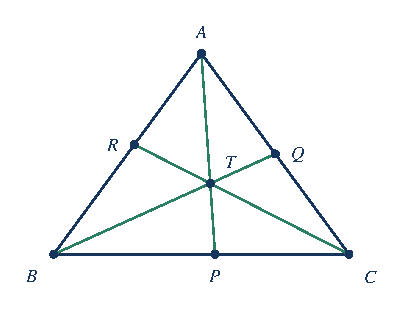
\includegraphics[width=.57\linewidth]{lb1-fig-09.pdf}
\FigureTag{LB1.9}{fig:lb1-09}
\end{figure}
Using brackets for areas,
\[
\frac{TP}{AP}=\frac{[BTP]}{[ABP]}=\frac{[TPC]}{[APC]}
=\frac{[BTP]+[TPC]}{[ABP]+[APC]}=\frac{[BTC]}{[ABC]}.
\]
Similarly,
$\dfrac{TP}{AP}+\dfrac{TQ}{BQ}+\dfrac{TR}{CR}
=\dfrac{[ATB]+[BTC]+[CTA]}{[ABC]}=1$.

Here is another application.
\paragraph{BAMO (2007).}
In triangle $ABC$, $D$ and $E$ are interior points on side $BC$ with $BD=CE$ and $\angle BAD=\angle CAE$.
Prove that $ABC$ is isosceles.
We use two elementary facts: triangles with equal bases and the same height have equal areas, and
$[ABC]=\frac12ab\sin A$.

% Source page 14 - left
Since $[ABD]=[AEC]$, we have
$\frac12\sin x\,AB\cdot AD=\frac12\sin x\,AC\cdot AE$, so $AB/AC=AE/AD$.
Also $BE=CD$ and $\angle BAE=\angle DAC$, whence $[ABE]=[ADC]$.
Thus
\[
\frac12\sin(x+z)\,AB\cdot AE=\frac12\sin(x+z)\,AC\cdot AD
\Longrightarrow\frac{AB}{AC}=\frac{AD}{AE}.
\]
It follows that $AD/AE=AE/AD$, so $AD=AE$ and $AB/AC=1$.
Therefore $ABC$ is isosceles.
\begin{figure}[H]\centering
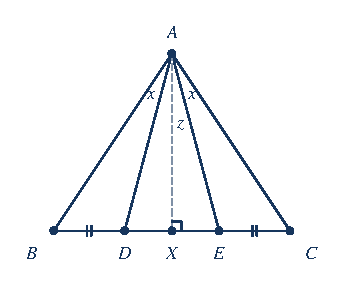
\includegraphics[width=.53\linewidth]{lb1-fig-10.pdf}
\FigureTag{LB1.10}{fig:lb1-10}
\end{figure}
\begin{remark}
Another major approach to geometry problems assigns masses to points and is sometimes called ``mass-point geometry.''
In my opinion, problems solved using these elementary operations on masses can be resolved using Ceva's theorem or Menelaus's theorem.
\end{remark}
The following is a nice application of Menelaus's theorem and can itself be considered a lemma.
\setcounter{theorem}{37}\begin{lemma}[Two concurrency conditions]
Let $ABC$ be a triangle, and let $D,E,F$ lie on $BC,CA,AB$, respectively, with $AD,BE,CF$ concurrent.
If $M,N,P$ lie on $EF,FD,DE$, then $AM,BN,CP$ concur if and only if $DM,EN,FP$ concur.
\end{lemma}
I used GeoGebra to draw a nice, neat figure of this problem. Do not forget Lemma~\ref{lemma:lb1-39} for if-and-only-if problems.
% Source page 14 - right
\begin{figure}[H]\centering
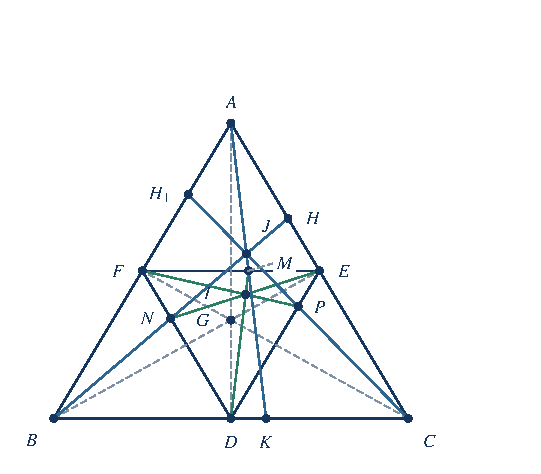
\includegraphics[width=.93\linewidth]{lb1-fig-11.pdf}
\FigureTag{LB1.11}{fig:lb1-11}
\end{figure}
\emph{``The secret of resolving any difficult geometric problem is drawing a clean figure.''}

\paragraph{Innovative solution.}
Let $D,E,F$ lie on the sides $BC,CA,AB$ of triangle $ABC$, respectively,
with $BD=CE=AF$ and $\angle BDF=\angle CED=\angle AFE$.
Prove that $ABC$ is equilateral.
\begin{figure}[H]\centering
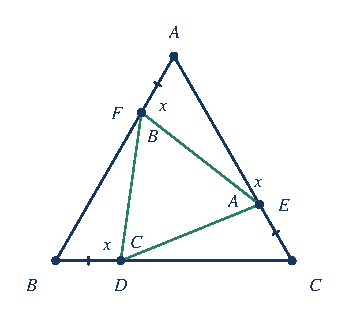
\includegraphics[width=.70\linewidth]{lb1-fig-17.pdf}
\FigureTag{LB1.17}{fig:lb1-17}
\end{figure}
Triangles $AFE,BFD,CED$ have equal bases and an equal angle.
If $A\geq B\geq C$, then $FE\geq FD\geq DE$.
Inside triangle $DEF$, $FD\geq DE\geq EF$.
Together these imply $FD=DE=EF$, hence $AB=BC=AC$.

\paragraph{Strategy: the poet's way.}
Temporarily assume the desired conclusion and work backwards to discover a useful intermediate claim. Then discard the assumption and prove that intermediate claim directly.

% Source page 33 - left
The following example illustrates this strategy.
\paragraph{Application: RMO (1995).}
In $\triangle ABC$, $K,L$ are points on $BC$ such that $BC\cdot KL=BK\cdot CL$, and $AL$ bisects $\angle KAC$.
Prove that $AL\perp AB$.
\begin{figure}[H]\centering
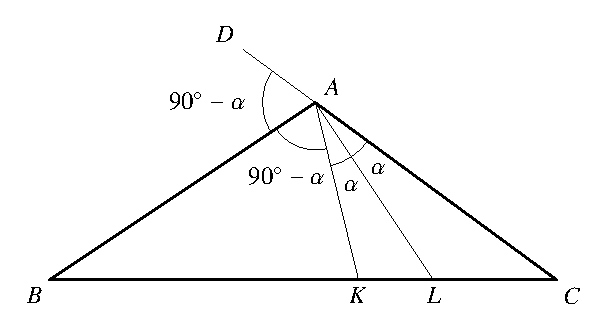
\includegraphics[width=.70\linewidth]{lb1-fig-18.pdf}
\FigureTag{LB1.18}{fig:lb1-18}
\end{figure}
Let us assume the result is true: $AL\perp AB$.
An angle chase then gives the needed intermediate relation.
Extend $CA$ beyond $A$ to a point $D$.
Since $AL$ bisects $\angle KAC$, let $\angle LAK=\angle LAC=\alpha$.
Then $\angle KAB=90^\circ-\alpha$ and
$\angle BAD=180^\circ-(90^\circ-\alpha+\alpha+\alpha)=90^\circ-\alpha$.
Thus $\angle KAB=\angle BAD=90^\circ-\alpha$, suggesting that $AB$ is an exterior angle bisector of $\triangle KAC$.
We now prove that fact independently. The hypothesis gives $BC/BK=CL/KL$, while the angle-bisector theorem gives $CL/KL=AC/AK$. Hence $BC/BK=AC/AK$, so the converse of the exterior angle-bisector theorem shows that $AB$ is the exterior angle bisector of $\angle KAC$.
The internal and exterior angle bisectors are perpendicular, so $AL\perp AB$.
This is exactly what we wanted.
% Source page 33 - right

Employ the same strategy to resolve the following problem.
In $\triangle ABC$, $AM$ is a median that divides $\angle BAC$ in the ratio
$1:2$. Extend $AM$ through $M$ to $D$ so that $\angle DBA=90^\circ$.
Prove that $AC=\tfrac12AD$.

\subsection{Solving geometry problems using scissors rather than theorems}
\paragraph{C.A.P.: Cut and Paste problem (IMO, 1996).}
Let $P$ be a point inside $\triangle ABC$ such that
\[\angle APB-\angle C=\angle APC-\angle B.\]
Let $D,E$ be the incentres of $\triangle APB,\triangle APC$, respectively.
Show that $AP,BE,CD$ concur.
% Source page 45 - left
\begin{figure}[H]\centering
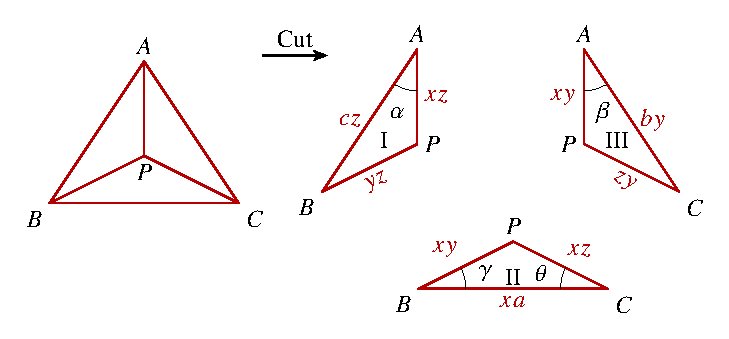
\includegraphics[width=.95\linewidth]{lb1-fig-23.pdf}
\FigureTag{LB1.23}{fig:lb1-23}
\end{figure}
Multiply the sides of triangle I by $z$, those of II by $x$, and those of III by $y$.
Anybody got some glue?! Okay, let's repaste.
\begin{figure}[H]\centering
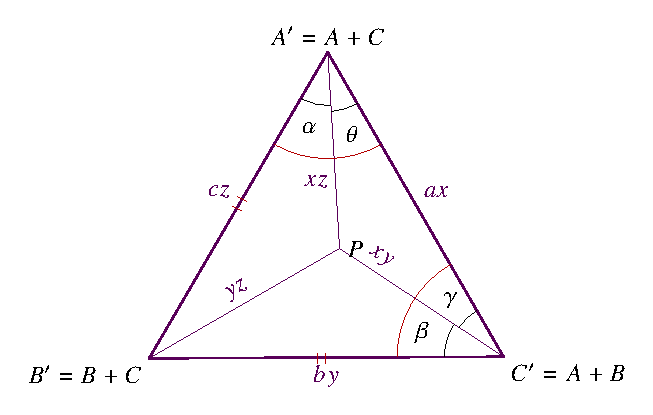
\includegraphics[width=.72\linewidth]{lb1-fig-24.pdf}
\FigureTag{LB1.24}{fig:lb1-24}
\end{figure}
The angle condition on $P$ gives $\alpha+\theta=\beta+\gamma$, so $cz=by$.
Thus $c/b=y/z$, giving $AB/AC=BP/CP$, and hence $AB/BP=AC/CP$.
This is the last step written in the source; the remaining argument proving the
requested concurrence of $AP,BE,CD$ is not supplied there.
% Source page 45 - right


\subsection{Two geometric constructions}
In $\triangle ABC$, $\angle A=120^\circ$.
Express the length of the internal angle bisector of $\angle A$ in terms of the two adjacent sides.
\begin{figure}[H]\centering
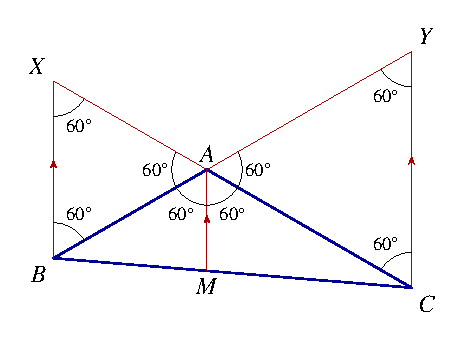
\includegraphics[width=.82\linewidth]{lb1-fig-25.pdf}
\FigureTag{LB1.25}{fig:lb1-25}
\end{figure}
The figure gives the required parallel lines: $X,A,C$ are collinear; $Y,A,B$ are collinear; and $XB\parallel AM\parallel YC$.
The construction is now clear from the figure, and the solution takes two lines:
\[\frac1{BX}+\frac1{CY}=\frac1{AM}
\quad\Longrightarrow\quad\frac1{AB}+\frac1{AC}=\frac1{AM}
\quad\Longrightarrow\quad AM=\frac{AB\cdot AC}{AB+AC}.\]
Q.E.D.!
% Source page 50 - right
In $\triangle ABC$, $CD$ is the altitude to $AB$, and $P$ is a point on $DC$.
$AP$ meets $CB$ at $Q$, and $BP$ meets $CA$ at $R$.
Prove that $\angle RDC=\angle QDC$ using Ceva's theorem.
\begin{figure}[H]\centering
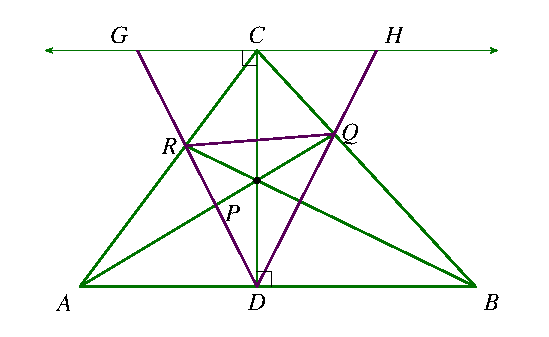
\includegraphics[width=.70\linewidth]{lb1-fig-26.pdf}
\FigureTag{LB1.26}{fig:lb1-26}
\end{figure}
Since $\triangle GRC\sim\triangle DRA$, we have $CR/RA=GC/AD$.
Also $\triangle CQH\sim\triangle BQD$, giving $BQ/CQ=BD/CH$.
Now Ceva's theorem yields
\[\frac{CR}{RA}\frac{AD}{DB}\frac{BQ}{QC}=1
\quad\Longrightarrow\quad\frac{GC}{AD}\frac{AD}{DB}\frac{BD}{CH}=1
\quad\Longrightarrow\quad CG=CH.\]
In $\triangle GCD$ and $\triangle HCD$, we have $GC=CH$ and $\angle GCD=\angle HCD=90^\circ$.
Thus $\triangle GDC\cong\triangle HDC$, so $\angle RDC=\angle QDC$.
Q.E.D.!
% BLOG-CONTENT-END
\end{document}
